\newpage
\section{Multidimensional Integrals}

\subsection{Arc-length of a Curve}

We will use the famous technique of approximating the length/area/volume of something
by dividing it in to equally smaller section that are straight lines in this case. In other will
be prisms, squares, etc. Now if we look at the difference between two points in our 3D space, 
for this Example
we notice that there are three differences \(\Delta i\) \(\Delta j\) \(\Delta k\).j
Now lets take the length of the vector \(\sqrt{{(\Delta i)}^2 + {(\Delta j)}^2 + {(\Delta k)}^2}\)

The total Arc-length is going to be the sum of all of this sectors
\[
L =  \sum_{i = 1}^{n}\sqrt{{(\Delta i)}^2 + {(\Delta j)}^2 + {(\Delta k)}^2}
\]

if we use a clever one we get

\[
L =  \sum_{i = 1}^{n}\sqrt{\frac{{\left(\frac{\Delta i}{\Delta t}\right)}^2 + {\left(\frac{\Delta j}{\Delta t}\right)}^2 + {\left(\frac{\Delta k}{\Delta t}\right)}^2}{\Delta t}}
\]

Now if we take the limit we get

\[
L =  \lim_{n\to \infty}\sum_{i = 1}^{n}\sqrt{\frac{{\left(\frac{\Delta i}{\Delta t}\right)}^2 + {\left(\frac{\Delta j}{\Delta t}\right)}^2 + {\left(\frac{\Delta k}{\Delta t}\right)}^2}{\Delta t}}
\]

which is 

\[
L =  \int_{a}^{b}\sqrt{{\left(\frac{\Delta i}{\Delta t}\right)}^2 + {\left(\frac{\Delta j}{\Delta t}\right)}^2 + {\left(\frac{\Delta k}{\Delta t}\right)}^2}\,dt
\]

\[
L =  \int_{a}^{b}\sqrt{{(f'(t))}^2 + {(g'(t))}^2 + {(h'(t))}^2}\,dt
\]

For differentiable function on the interval \(t \in [a; b]\)

\subsection{Line Integrals}

\subsubsection{Over Vector Field}

Let \( F : \mathbb{R}^n \to \mathbb{R}^n \) be a vector field, and let \( \gamma \) be a smooth curve parametrized by \( \vec{r}(t) \), \( t \in [a, b] \). The \emph{line integral} of \( F \) 
along \( \gamma \) is:

\[
\int_\gamma \langle \nabla \vec{F}, d\vec{r} \rangle = \int_a^b \langle \vec{F}(\vec{r}(t)), \vec{r}'(t) \rangle \, dt = \vec{F}(\vec{r}(b)) - \vec{F}(\vec{r}(a))
\]

In the context of physics this integral measures the work done by the field \( \vec{F} \) along the path \( \gamma \), such as force over distance.

\subsection{Over Scalar field}

Let \( f(x_1, x_2, \ldots, x_n) \) be a scalar field defined on a smooth curve \( C \), which is parameterized by a vector function

\[
\vec{r}(t) = (x_1(t), x_2(t), \ldots, x_n(t)), \quad t \in [a, b]
\]

Then, the line integral of \( f \) over \( C \) is given by:

\[
\int_C f(x_1, x_2, \ldots, x_n) \, ds = \int_a^b f(\vec{r}(t)) \left\| \vec{r}'(t) \right\| \, dt
\]


\begin{center}
    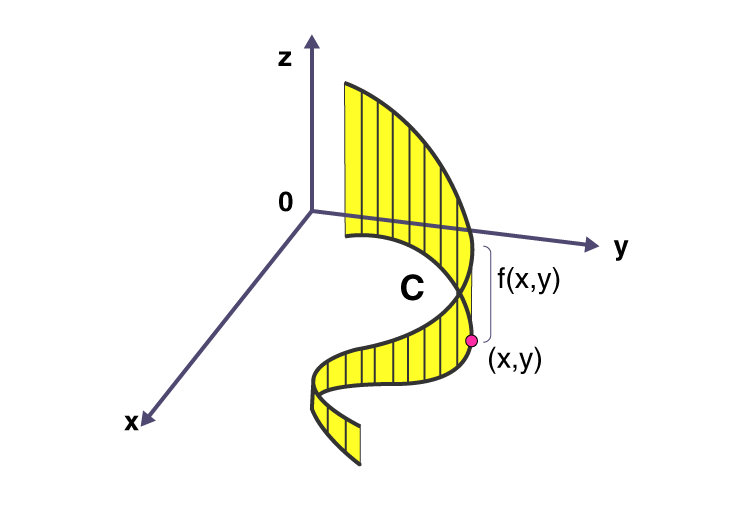
\includegraphics[width=0.5\textwidth]{Line-integral.png}
\end{center}

\textbf{Example: Scalar Field}
\vspace{\baselineskip}

Compute the line integral of \(f(x,y) = x^2 + y^2\) over the straight line segment going
from \((1,1)\) to \((3,3)\)
\\
This time or curve is \(y = x\) to the parametrized curve is \(\begin{pmatrix}
    x(t) = t \\ y(t) = t
\end{pmatrix}\) this left us with:

\[
\int_{1}^{3}  2t^2 \sqrt{2}dt = \frac{52\sqrt{2}}{3} 
\]

\textbf{Example: Line Integral over a Vector Field}
\vspace{\baselineskip}

Let \( f(x, y) = x^2 + y^2 \), and define a vector field based on its gradient:

\[
\vec{F}(x, y) = \nabla f(x, y) = \left( \frac{\partial f}{\partial x}, \frac{\partial f}{\partial y} \right) = (2x, 2y)
\]

Let the curve \( C \) be the quarter-circle of radius 1 from \( (1, 0) \) to \( (0, 1) \), parameterized by:

\[
\vec{r}(t) = (\cos t, \sin t), \quad t \in \left[0, \frac{\pi}{2}\right]
\]

We compute the line integral of \( \vec{F} \) along \( C \):

\[
\int_C \langle \vec{F}, d\vec{r}\rangle = \int_0^{\frac{\pi}{2}} \langle\vec{F}(\vec{r}(t)) \vec{r}'(t) \rangle\, dt
\]

First, compute:

\[
\vec{F}(\vec{r}(t)) = (2\cos t, 2\sin t), \quad \vec{r}'(t) = (-\sin t, \cos t)
\]

Now compute the dot product:

\[
\langle\vec{F}(\vec{r}(t)), \vec{r}'(t)\rangle = 2\cos t \cdot (-\sin t) + 2\sin t \cdot \cos t = -2\cos t \sin t + 2\cos t \sin t = 0
\]

Therefore, the line integral is:

\[
\int_C \langle \vec{F}, d\vec{r}\rangle = \int_0^{\frac{\pi}{2}} 0 \, dt = 0
\]

The line integral of the gradient vector field \( \vec{F} = \nabla f \) over this curve is zero. 
This is consistent with the fact that line integrals of gradient fields over 
curves depend only on endpoints, and 
\( f(1,0) = 1 \), \( f(0,1) = 1 \), so \( f(B) - f(A) = 0 \).


\subsection{Potential Function}

A vector field \( \vec{F} : \mathbb{R}^n \to \mathbb{R}^n \) is called \emph{conservative} if there exists a scalar function \( \phi : \mathbb{R}^n \to \mathbb{R} \) such that:

\[
\vec{F} = \nabla \phi
\]

The function \( \phi \) is then called a \emph{potential function} of \( \vec{F} \).

\textbf{Properties:}
\begin{itemize}[label=\(-\)]
    \item The line integral of \( \vec{F} \) over any path depends only on the endpoints:
    \[
    \int_\gamma \langle \vec{F}, d\vec{r} \rangle = \phi(B) - \phi(A)
    \]
    \item The line integral over a closed path is zero:
    \[
    \oint_\gamma \langle \vec{F}, d\vec{r} \rangle = 0
    \]
    \item \( \vec{F} \) is conservative \( \Leftrightarrow \) \( \vec{F} \) has zero curl in a simply connected region.
\end{itemize}

\subsection{Finding the Potential Function of a Vector Field}

To find the potential function \( \phi(x, y) \) of a vector field \( \vec{F}(x, y) = (P(x, y), Q(x, y)) \), we must check if the field is conservative and then integrate accordingly. A vector field is conservative if there exists a scalar potential function \( \phi \) such that:
\[
\vec{F} = \nabla \phi = \left( \frac{\partial \phi}{\partial x}, \frac{\partial \phi}{\partial y} \right)
\]

\textbf{Given:}
\[
\vec{F}(x, y) = \left(2xy + e^x,\ x^2 + \frac{1}{2\sqrt{y}}\right)
\]

Let \( P(x, y) = 2xy + e^x \), and \( Q(x, y) = x^2 + \frac{1}{2\sqrt{y}} \).

First, check if the field is conservative by verifying:
\[
\frac{\partial P}{\partial y} = \frac{\partial}{\partial y}(2xy + e^x) = 2x
\]
\[
\frac{\partial Q}{\partial x} = \frac{\partial}{\partial x}\left(x^2 + \frac{1}{2\sqrt{y}}\right) = 2x
\]

Since \( \frac{\partial P}{\partial y} = \frac{\partial Q}{\partial x} \), the field is conservative.
\vspace{\baselineskip}

\textbf{Step 1: Integrate \( P(x, y) \) with respect to \( x \):}
\[
\phi(x, y) = \int (2xy + e^x)\,dx = x^2y + e^x + h(y)
\]
Here, \( h(y) \) is a function of \( y \) only.
\vspace{\baselineskip}

\textbf{Step 2: Differentiate \( \phi(x, y) \) with respect to \( y \):}
\[
\frac{\partial \phi}{\partial y} = x^2 + h'(y)
\]

Set this equal to \( Q(x, y) = x^2 + \frac{1}{2\sqrt{y}} \), so:
\[
x^2 + h'(y) = x^2 + \frac{1}{2\sqrt{y}} \Rightarrow h'(y) = \frac{1}{2\sqrt{y}}
\]

\textbf{Step 3: Integrate to find \( h(y) \):}
\[
h(y) = \int \frac{1}{2\sqrt{y}}\,dy = \sqrt{y} + C
\]

\textbf{Final potential function:}
\[
\phi(x, y) = x^2y + e^x + \sqrt{y} + C
\]

Therefore, the potential function is:
\[
\boxed{\phi(x, y) = x^2y + e^x + \sqrt{y} + C}
\]


\subsection{Double Integral over a Rectangular Region}

Let \( A = [x_0, x_1] \times [y_0, y_1] \) be a rectangular region in \( \mathbb{R}^2 \). The double integral of a function \( f(x, y) \) over \( A \) is:

\[
\iint_A f(x, y)\, dA = \int_{x_0}^{x_1} \int_{y_0}^{y_1} f(x, y)\, dy\, dx
\]

For rectangular domains, the order of integration does not affect the result:

\[
\int_{x_0}^{x_1} \int_{y_0}^{y_1} f(x, y)\, dy\, dx = \int_{y_0}^{y_1} \int_{x_0}^{x_1} f(x, y)\, dx\, dy
\]


\subsection{Integration over Curvilinear Domains}

If the region \( A \subset \mathbb{R}^2 \) is not rectangular, it is divided into subregions \( \Delta A_k \), and the integral is defined as the limit:

\[
\iint_A f(x, y)\, dA = \lim_{n \to \infty} \sum_{k=1}^n f(x_k, y_k) \, \Delta A_k
\]

In practice, for regions bounded by curves, we integrate in the form:
\[
\int_a^b \int_{u(x)}^{o(x)} f(x, y)\, dy\, dx
\]

Here, \( y \in [u(x), o(x)] \) describes the vertical bounds as functions of \( x \).
\vspace{\baselineskip}

\textbf{Example:}
\vspace{\baselineskip}

Compute the volume under \(f(x,y) = 1 + x + y^2\) bounded by \(x\)-axis, \(x = 1\) and \(y\)-axis \(y = \sqrt{x}\)

\begin{center}
    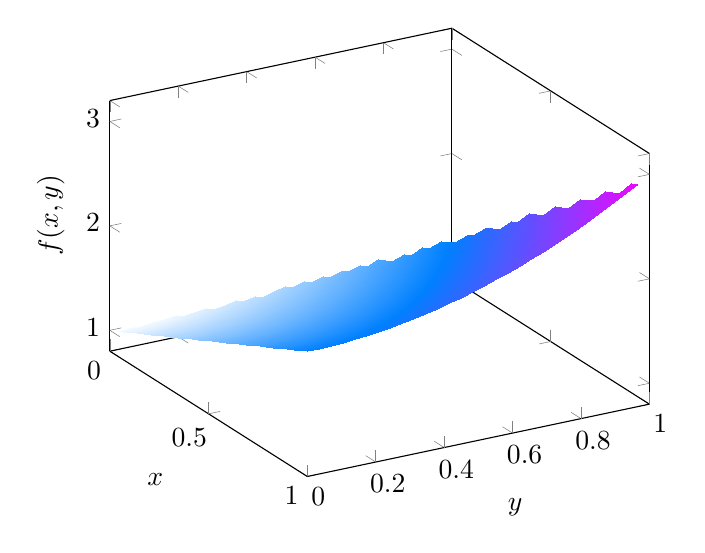
\begin{tikzpicture}
        \begin{axis}[
            view={60}{30},
            xlabel=$x$,
            ylabel=$y$,
            zlabel={$f(x,y)$},
            domain=0:1,
            y domain=0:1,
            samples=30,
            samples y=30,
            colormap/cool,
        ]
            \addplot3 [
                surf,
                domain=0:1,
                y domain=0:1,
                samples=30,
                samples y=30,
                restrict z to domain=-10:10,
                shader=interp,
            ]
            {y <= sqrt(x) ? 1 + x + y^2 : NaN};
        \end{axis}
    \end{tikzpicture}
\end{center}

First we are going to imagine slicing the area under this sector vertically along the \(x\)-axis from \(0\) up to \(1\) which
is the volume of an Area under a curve that is represented by going along the \(y\)-axis.

\begin{align*}
    \int_{0}^{1}\int_{0}^{\sqrt{x}} 1 + x + y^2 dy dx \\
    \int_{0}^{1} \left| y + xy + \frac{y^3}{3} \right|_{0}^{\sqrt{x}} dx \\
    \int_{0}^{1} \left| \sqrt{x} + x\sqrt{x} + \frac{\sqrt{x}^3}{3} \right|_{0}^{\sqrt{x}} dx \\
    = \left| \frac{2}{3} x^{\frac{3}{2}} + \frac{4}{3} \frac{2}{5} x^{\frac{5}{2}} \right|_{0}^{1} = \frac{6}{5}
\end{align*}

If we choose the other way then we have an area with a fix \(y\) in the inside that goes from \(y^2\) to \(1\) with respect to \(x\).
\[
\int_{0}^{1}\int_{y^2}^{1} 1 + x + y^2 dx dy
\]

\subsection{Changing the order of integration to solve tricky integrals}

Given \(\int_{0}^{8}\int_{\sqrt[3]{x}}^{2} \frac{1}{y^4 +1}dy dx\) which is very hard to integrate, lets change the order
to make it easier.

\[\int_{0}^{2}\int_{0}^{y^3} \frac{1}{y^4 +1}dx dy\]

The steps are the same as in the previous Example.

\begin{enumerate}
    \item Identify the area you want to integrate, what are the bounds respective to \(x\) and \(y\)
    \item Write the same expression without bounds and change the order of the differentials
    \item Imagine slicing the area underneath vertically for \(x\) and horizontally for \(y\) with their respective bounds corresponding
    to the perspective.
    \item Write the new integral with the opposite of order of integration
\end{enumerate}

\begin{center}

    Visualization of the area underneath the surface
    \smallskip

    \begin{tikzpicture}
        \begin{axis}[
            axis lines=middle,
            xlabel={$x$},
            ylabel={$y$},
            legend pos=outer north east,
            domain=0:8,
            samples=200
        ]
            % Shading the area between the two functions
            \addplot [
                name path=A,
                domain=0:8,
                samples=200,
                draw=none
            ] {pow(x, 1/3)};
            
            \addplot [
                name path=B,
                domain=0:8,
                samples=200,
                draw=none
            ] {2};

            \addplot [
                orange,
                fill opacity=0.3
            ] fill between[of=A and B];

            % Plot both functions
            \addplot[color=black, domain=0:8, samples=200]{pow(x, 1/3)};

            \addplot[color=blue, dashed, domain=0:8, samples=200]{2};

        \end{axis}
    \end{tikzpicture}
\end{center}

Here the original bounds are: \(x\) goes from 0 to 8 and \(y\) goes from \(\sqrt[3]{x}\) to 2.
As you can see in the diagram by slicing vertically the value of \(x\) is fixed and we move towards the upper-bound of \(y\) which is 2.
Therefore the smallest \(x\) can get is 0 and the biggest is 2. While for \(y\) by slicing vertically we get that \(x\) goes from 0
to \(\sqrt[3]{x}\) but we do not want to left that y so we solve for y and get \(y^3\). Now we caput all of this together and integrate.


\subsection{The Jacobian}

The Jacobian matrix is a fundamental concept in multi-variable calculus. The Jacobian is best
approximation of a linear transformation for a point.

For the intuition of why, we use partial derivatives, just think about
how we use them as this tiny changes in the component of original
basis vectors.

Given a vector-valued function

\[
\mathbf{f} : \mathbb{R}^n \rightarrow \mathbb{R}^m, \quad f(x_1, \ldots, x_n) = 
\begin{bmatrix}
f_1(x_1, \ldots, x_n) \\
f_2(x_1, \ldots, x_n) \\
\vdots \\
f_m(x_1, \ldots, x_n)
\end{bmatrix},
\]
the \emph{Jacobian matrix} of \(f\) is the \(m \times n\) matrix of all first-order partial derivatives:
\[
J_f(x) = \begin{bmatrix}
\frac{\partial f_1}{\partial x_1} & \frac{\partial f_1}{\partial x_2} & \cdots & \frac{\partial f_1}{\partial x_n} \\
\frac{\partial f_2}{\partial x_1} & \frac{\partial f_2}{\partial x_2} & \cdots & \frac{\partial f_2}{\partial x_n} \\
\vdots & \vdots & \ddots & \vdots \\
\frac{\partial f_m}{\partial x_1} & \frac{\partial f_m}{\partial x_2} & \cdots & \frac{\partial f_m}{\partial x_n}
\end{bmatrix}.
\]

\subsubsection{Local linearity}
While performing non linear transformations on a space. We can see that in a tiny neighborhood
around a point, the transformation appears to be linear. And the matrix that encodes that
transformation is the \emph{Jacobian}.

For intuition, just imagine that in the tiny neighborhood the transformation is composed
of a small steps in the \(x_1, \dots, x_n\) directions which give of the partial derivatives that
represent this small steps. 

\subsubsection{Determinant}
When \(m = n\), i.e., the function maps from 
\(\mathbb{R}^n\) to \(\mathbb{R}^n\), 
the Jacobian matrix is square. In this case, 
the \textit{Jacobian determinant} is defined as:
\[
\det(J_{f}(x)),
\]
and provides important information about the local behavior of the function. For instance:
\begin{itemize}[label=\(-\)]
  \item If \(\det(J_{f}(x)) \neq 0\), the function is locally invertible at \(x\) by the inverse 
  function theorem.
  \item The sign and magnitude of the determinant 
  inform about orientation and volume scaling of the transformation.
\end{itemize}

When we change our systems of coordinates it is important
that our differential make sense in the original system we were.
Because of that, we take the determinant with respect to the new
coordinates to tell us the scaling factor that we have to use for our
result to make sense.
\vspace{\baselineskip}

\textbf{Use Cases}
\vspace{\baselineskip}

The Jacobian matrix and its determinant appear in many areas, including:
\begin{itemize}[label=\(-\)]
  \item \textbf{Change of variables in integrals:} The absolute value of the Jacobian determinant is used to adjust the measure when changing coordinates in multiple integrals.
  \item \textbf{Nonlinear optimization:} The Jacobian is crucial for computing gradients and performing techniques like Newton's method in multiple dimensions.
  \item \textbf{Differential equations:} Stability analysis of dynamical systems often involves evaluating the Jacobian at equilibrium points.
\end{itemize}

\subsubsection{List of Common Jacobians}

\begin{itemize}[label=\(-\)]

    \item \emph{Cartesian Coordinates}:
    \begin{itemize}[label=\(-\)]
        \item Definition: The position of a point is given by \((x, y, z)\) in a 3D space along orthogonal axes.
        \item Jacobian: 
        \[
        J_{\text{Cartesian}} = 1dx
        \]
    \end{itemize}

    \item \emph{Polar Coordinates (2D)}:
    \begin{itemize}[label=\(-\)]
        \item Definition: The position of a point in a plane is given by \((r, \theta)\), where \(r\) is the radial distance and \(\theta\) is the angle from the positive \(x\)-axis.
        \item Jacobian:
        \[
        J_{\text{Polar}} = rd rd\theta
        \]
    \end{itemize}

    \item \emph{Cylindrical Coordinates}:
    \begin{itemize}[label=\(-\)]
        \item Definition: The position of a point in 3D space is given by \((r, \theta, z)\), where \((r, \theta)\) are the polar coordinates in the \(xy\)-plane and \(z\) is the height along the \(z\)-axis.
        \item Jacobian:
        \[
        J_{\text{Cylindrical}} = r\ dr d\theta dz
        \]
    \end{itemize}

    \item \emph{Spherical Coordinates}:
    \begin{itemize}[label=\(-\)]
        \item Definition: The position of a point in 3D space is given by \((\rho, \theta, \phi)\), where:
        \begin{itemize}[label=\(-\)]
            \item \(\rho\) is the distance from the origin,
            \item \(\theta\) is the azimuthal angle (in the \(xy\)-plane from the positive \(x\)-axis),
            \item \(\phi\) is the polar angle (from the positive \(z\)-axis).
        \end{itemize}
        \item Jacobian:
        \[
        J_{\text{Spherical}} = \rho^2 \sin (\phi) d\rho d\theta d\phi
        \]
    \end{itemize}

\end{itemize}

\subsection{Integration in Polar Coordinates}

For radially symmetric regions or functions, switching to polar coordinates simplifies the computation.
\vspace{\baselineskip}

\textbf{Transformation:}
\[
x = r \cos \varphi, \quad y = r \sin \varphi
\]

The Jacobian of the transformation gives the area element:
\[
dA = r\, dr\, d\varphi
\]


\emph{Integral:}
\[
\iint_D f(x, y)\, dA = \int_{\varphi_0}^{\varphi_1} \int_{0}^{R(\varphi)} f(r \cos \varphi, r \sin \varphi)\, r\, dr\, d\varphi
\]

\subsubsection{Origin of the Area}
When we divide our circle in the sections we get both a difference in then angle and the radius which generate another area.
The difference \(\Delta A =\) Area of big wedge \(-\) Area of small wedge
\vspace{\baselineskip}

\emph{Radius: }\(r_k + \frac{\Delta r}{2}\) for the big wedge and \(r_k - \frac{\Delta r}{2}\) for the small wedge
\vspace{\baselineskip}

\emph{Angle: }\(\frac{\Delta \theta}{2 \pi}\) which is the angle of the fraction of the circle because the formula for the area is \(r^2 \pi\)
and the whole circle would be \(2\pi\)
\vspace{\baselineskip}

\emph{Final Formula for the difference in the Area}

\[\Delta A = \frac{\Delta \theta}{2 \pi} \left ( {\left[r_k + \frac{\Delta r}{2}\right]}^2 - {\left[r_k - \frac{\Delta r}{2}\right]}^2\right)\] 
\[ = r_k \Delta r \Delta \theta\]

Which multiplied by the function value and by taking the limit of this sections we get that the volume:

\[
V = \int_{\theta_1}^{\theta_2} \int_{r_1 (\theta)}^{r_2 (\theta)} f(r, \theta) r \Delta r \Delta \theta
\]

\textbf{Example:}
\vspace{\baselineskip}

\(f(r, \theta) = r\) above cardioid \(r = 1 - \sin \theta\)

Then

\[
V = \int_{0}^{2\pi}\int_{0}^{1 - \sin \theta} r r dr d\theta
\]

\[
= \int_{0}^{2\pi}\frac{r^3}{3} |_{0}^{1 - \sin \theta} d\theta = \int_{0}^{2\pi} \frac{{(1 - \sin\theta)}^3}{3} d\theta = \frac{5 \pi}{3}
\]


\subsection{Improper Integrals over Unbounded Regions}

If the domain of integration is unbounded (e.g., the entire plane \( \mathbb{R}^2 \)), the double integral is defined via a limit process:

\[
\iint_{\mathbb{R}^2} f(x, y)\, dx\, dy := \lim_{M_1, M_2 \to \infty} \lim_{N_1, N_2 \to \infty}
\int_{M_1}^{M_2} \int_{N_1}^{N_2} f(x, y)\, dy\, dx
\]

Often, using polar coordinates simplifies such cases, reducing multiple limits to one:

\[
\iint_{\mathbb{R}^2} f(x, y)\, dx\, dy = \int_0^{2\pi} \int_0^{\infty} f(r \cos \varphi, r \sin \varphi)\, r\, dr\, d\varphi
\]


\subsubsection{Gaussian Integral}

We are going to find the integral of the \emph{unbounded integral} 
\(e^{-x^2}\)using a combination of techniques.

\begin{align*}
S &= \int_{-\infty}^{\infty} e^{-x^2}dx\\
S^2 &= \left(\int_{-\infty}^{\infty} e^{-x^2}dx\right) \left(\int_{-\infty}^{\infty} e^{-x^2}dx\right)\\
S^2 &= \left(\int_{-\infty}^{\infty} e^{-x^2}dx\right) \left(\int_{-\infty}^{\infty} e^{-y^2}dy\right)
\end{align*}

Now lets translate to polar coordinates

\begin{align*}
S^2 &= \left(\int_{0}^{2\pi} \int_{0}^{\infty}re^{-{(r\cos\theta)}^2} re^{-{(r\sin\theta)}^2}drd\theta\right)\\
S^2 &= \left(\int_{0}^{2\pi} \int_{0}^{\infty}re^{-{(r\cos\theta)}^2 + {(r\sin\theta)}^2}drd\theta\right)\\
S^2 &= \left(\int_{0}^{2\pi} \int_{0}^{\infty}re^{-(r^2)}drd\theta\right)\\
S^2 &=  \left(\int_{0}^{2\pi} \int_{0}^{\infty}\frac{1}{2}e^{-(s)}dsd\theta\right)\\
S^2 &= \left(\int_{0}^{2\pi}d\theta\right)\\
S^2 &= \pi\\
S   &= \sqrt{\pi}
\end{align*}

\QED

\subsection{Triple Integrals}

The triple integral allows the computation of volume or mass in three-dimensional space.

Let \( V \subset \mathbb{R}^3 \) be a bounded region, then:

\[
\iiint_V f(x, y, z)\, dV = \lim_{n \to \infty} \sum_{k=1}^n f(x_k, y_k, z_k) \, \Delta V_k
\]

where \( \Delta V_k \) are small sub-volumes approximating \( V \).

In practice, evaluate:
\[
\iiint_V f(x, y, z)\, dz\, dy\, dx
\]

with limits determined by the geometry of the volume. The order of integration may be rearranged to simplify computation.

\[
\int_{x=a}^{x=b}\int_{y=g_1(x)}^{y=g_2(x)} \int_{f_1(x,y)}^{f_2(x,y)} dz dy dx
\]

\subsubsection{Triple Integrals in Cartesian Coordinates}

In this short section we, will look at an example of how to calculate the volume enclose in
between two functions using triple integrals.

Given are the functions \(f_1(x,y) = x^2 + y^2\) and \(f_2(x,y) = 3 - x^2 - y^2\)


\begin{center}
    
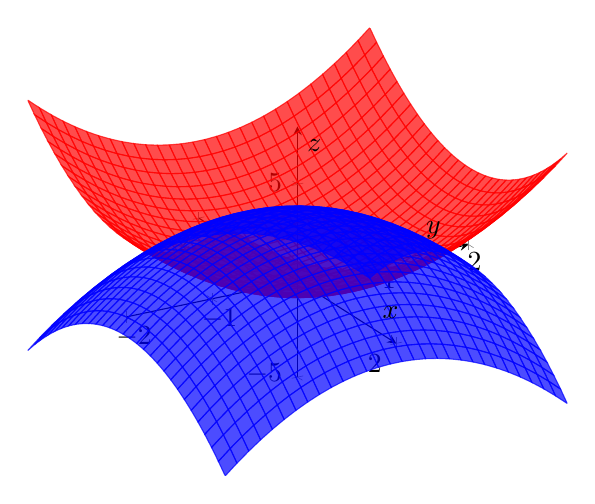
\begin{tikzpicture}
    \centering
    \begin{axis}[
        view={60}{30},
        axis lines=center,
        xlabel=$x$, ylabel=$y$, zlabel=$z$,
        domain=-2:2,
        y domain=-2:2,
        samples=30,
        samples y=30,
        colormap/jet,
    ]
        % Plot f1(x,y) = x^2 + y^2 in red
        \addplot3[
            surf,
            shader=flat,
            draw=red,
            fill=red,
            opacity=0.7,
        ]
        {x^2 + y^2};
    
        % Plot f2(x,y) = 3 - x^2 - y^2 in blue
        \addplot3[
            surf,
            shader=flat,
            draw=blue,
            fill=blue,
            opacity=0.7,
        ]
        {3 - x^2 - y^2};
    \end{axis}
\end{tikzpicture}
\end{center}

Lets find the intersection

\[
x^2 + y^2 = 3 -x^2 - y^2 
\]
\[
x^2 + y^2 = \frac{3}{2}
\]

Now we have to find the limits of integration for 
\[
\int_{x=a}^{x=b}\int_{y=g_1(x)}^{y=g_2(x)} \int_{f_1(x,y)}^{f_2(x,y)} dz dy dx
\]

using our constraint and our original functions.

\[
\int_{x=a}^{x=b}\int_{y=-\sqrt{\frac{3}{2} - x^2}}^{\sqrt{\frac{3}{2} -x^2}} \int_{x^2 + y^3}^{3-x^2-y^2} dz dy dx
\]

Here \(z\) means the height which is just the output
of the original functions.

The bounds of \(y\) just by looking at out constraint and solving for it.

And \(x\) only depends on the concrete limit of integration.


\subsubsection{Coordinate Transformation and the Jacobian Determinant}

Let a coordinate transformation be defined by:
\[
x = x(u, v, w), \quad y = y(u, v, w), \quad z = z(u, v, w)
\]

Then the triple integral transforms as:
\[
\iiint_{(x, y, z)} f(x, y, z)\, dx\, dy\, dz = \iiint_{(u, v, w)} f(x(u, v, w), y(u, v, w), z(u, v, w)) \cdot \left| \det J \right|\, du\, dv\, dw
\]

where \( J \) is the \emph{Jacobian matrix} of the transformation:
\[
J = 
\begin{pmatrix}
\frac{\partial x}{\partial u} & \frac{\partial x}{\partial v} & \frac{\partial x}{\partial w} \\
\frac{\partial y}{\partial u} & \frac{\partial y}{\partial v} & \frac{\partial y}{\partial w} \\
\frac{\partial z}{\partial u} & \frac{\partial z}{\partial v} & \frac{\partial z}{\partial w}
\end{pmatrix}
\]

\textbf{Example: Transformation to Cylindrical Coordinates}

The standard cylindrical coordinate transformation is:
\[
x = r \cos \varphi, \quad y = r \sin \varphi, \quad z = z
\]

The Jacobian determinant is:
\[
\left| \det J \right| =
\begin{vmatrix}
\cos \varphi & -r \sin \varphi & 0 \\
\sin \varphi & r \cos \varphi & 0 \\
0 & 0 & 1
\end{vmatrix}
= r
\]

Thus, the triple integral in cylindrical coordinates becomes:
\[
\iiint f(x, y, z)\, dx\, dy\, dz = \iiint f(r \cos \varphi, r \sin \varphi, z)\, r\, dr\, d\varphi\, dz
\]

\subsubsection{Calculating the center of mass with triple integrals}

We can make use of triple integration to calculate the center of mass of a body with
respect to \(x\), \(y\) or \(z\) with the following formulas:

\[x_s = \iiint_V xp(x,z,y)dz\ dy \ dx\]
\[y_s = \iiint_V yp(x,z,y)dz\ dy \ dx\]
\[z_s = \iiint_V zp(x,z,y)dz\ dy \ dx\]

Where \(p(x,y,z)\) is our mass function.
